\documentclass{article}
\usepackage{graphicx} % Required for inserting images
\usepackage{amsmath}
\usepackage{amssymb}
\usepackage{tikz}
\usepackage{caption}
\usepackage[a4paper, left=1in, right=1in, top=1in, bottom=1in]{geometry}
\usepackage{chemfig}
\usepackage{cancel}
\usepackage{pgfplots}
\title{Estatística}
\author{Daniel Vital}
\date{November 2024}

\begin{document}

\maketitle

\section{Probabilidades Finitas dos Espaços Amostrais Finitos}
Seja S um espaço amostral finito $S=\{a_1\;,a_2\;,...a_n\}$, considere o evento de resultado simples\\$A=\{a_i\}$. Para cada evento simples $\{a_i\}$, existe uma probabilidade associada $P_i$, que satisfaz as aseguintes condições:
\begin{itemize}
    \item $p_i\geq 0\;\;\;\;\;\;\;\; i=1,2,...,n$
    \item $p_1+p_2+p_3+...+p_n=1$
\end{itemize}
A probabilidade $P(A)$ de um evento com mais de um elemento (evento composto), é definida pela soma das probabilidades de seus pontos.\\
Os eventos não tem, necessariamente, a mesma probabilidade.\\
Não há interseção entre os eventos\\

Exemplo: Sejam três cavalos de corrida ``A", ``B" e ``C", onde:\\
``A" tem 2x mais probabilidade de ganhar que ``B"\\
``B" tem 2x mais probabilidade de ganhar que ``C"\\

a) Qual a probabilidade de vitória de cada um?\\
$P(C) = P \;\;\;\;\;\; P(B)= 2P \;\;\;\;\;\; P(A)= 2\cdot(2P)=4P$\\

\noindent{$P + 2P + 4P =1$}\\
$7P=1\\
P=\frac{1}{7}$\\

$P(C) = \frac{1}{7}\;\;\;\;\; P(B)=\frac{2}{7} \;\;\;\;\; P(A)= \frac{4}{7}$
\\\\


b) Qual a probabilidade de B \textbf{ou} C ganharem?\\
$P(B\cup P)=P(B)+P(C)$\\
$P(A \cup B)= \frac{2}{7} + \frac{1}{7}\;\;\;\;\;\;\;\;\; \therefore  \;\;P(A \cup B) = \frac{3}{7}$\\

\noindent{ATENÇÃO: Para calcular a probabilidade nesse caso, é usada soma e não multiplicação, pois são eventos mutuamente exclusivos, não podem ocorrer ao mesmo tempo.}\\

\newpage
\section{Espaços Amostrais Finitos e Equiprováveis}
Espaço amostral Equiprovável ou Uniforme: Quando cada ponto amostral tem a mesma probabilidade.\\
Se $S$ possui $n$ pontos, a probabilidade de cada ponto é \\
\[\displaystyle p=\frac{1}{n}\]
Se um evento \textit{A} contem $r$ pontos, então:
\[P(A)=r\cdot\frac{1}{n}=\boxed{\frac{r}{n}}\]\\
\indent Essa fórmula pode, também, ser escrita como:\\
\[P(A)=\frac{\text{Nº de vezes que ``A'' pode ocorrer}}{\text{Nº de vezes que o espaço amostral ``S'' ocorre}}\]
\indent Ou
\[P(A)=\frac{\text{NCF (Nº de casos favoráveis)}}{\text{NTC (Nº total de casos)}}\hspace{.7cm}=\;\;\;\;\;\frac{r}{n}\]\\

\noindent Exemplo: David \underline{randomly} (``Aleatório'' indica que o espaço é equiprovável!) chose one card from a deck of 52 cards. What is the probability of ``A''? What is the probability of ``B''?\\
$A=\{\text{A carta é de ouros}\}$\\
$B=\{\text{A carta é uma figura}\}$\\
\[P(A)= \frac{\text{Nº de ouros}}{\text{Nº de cartas}}=\frac{13}{52}=\frac{1}{4} \;\;\;\;\;\;\;;\;\;\;\;\;\; P(B)=\frac{\text{Nº de figuras}}{\text{Nº de cartas}}=\frac{12}{52}=\frac{3}{13}\]\\
\\Como se observa, o cálculo de probabilidade está intimamente ligado a um problema de contagem, então usaremos análise combinatória para contabilizar casos totais e favoráveis.\\

{\large Análise Combinatória}\\
\[C_{n,p}=\binom{n}{p}=\frac{n!}{p!(n-p)!}\]\\
\indent Exemplo: Quantas comissões de 3 pessoas são possíveis formar a partir de um grupo de 10 pessoas?\\
\[C_{10,3}=\binom{10}{3}=\frac{10!}{3!(10-3)!}=120\]\\

{\large Espaços Amostrais Finitos e equiprováveis - Exercício:}\\

\noindent Num lote de 12 peças, 4 são defeituosas. Duas peças são escolhidas aleatoriamente\\
\textbf{a) Qual a probabilidade de ambas serem defeituosas?}\\

\noindent A=\{ambas são defeituosas\}\\
A pode ocorrer $\binom{4}{2}=C_{4,2}=\frac{4!}{2!\cdot2!}=6$ vezes \hspace{1.5cm} $\therefore \boxed{P(A)=\frac{NCF}{NTC}=\frac{6}{66}=\frac{1}{11}}$\\

\noindent S pode ocorrer $\binom{12}{2}=C_{12,2}=\frac{12!}{2!\cdot10!}=66$ vezes\\

\noindent \textbf{b) Probabilidade de ambas serem defeituosas}\\

\noindent B=\{Ambas não possuírem defeitos defeituosas\}\\
\noindent B pode ocorrer $\binom{8}{2}=C_{8,2}=\frac{8!}{2!\cdot6!}=28$\hspace{1.5cm} $\therefore \boxed{P(B)=\frac{NCF}{NTC}=\frac{28}{66}=\frac{14}{33}}$\\

\noindent S pode ocorrer $\binom{12}{2}=C_{12,2}=\frac{12!}{2!\cdot10!}=66$ vezes
\newpage
\noindent \textbf{c) Probabilidade de ao menos uma ser defeituosa}\\

\noindent C=\{ao menos uma é defeituosa\}\\

\noindent C é o complemento de B, ou seja, C=$\overline{B}$, pois:\\
Se tirarmos os pontos em que ambas as peças não possuem defeitos (B), no espaço amostral só sobrarão os pontos em que uma ou mais são defeituosas (que é equivalente a $\overline{B}$, que satisfaz C)\\

\noindent $\displaystyle\therefore P(C)= 1-P(B)=1-\frac{14}{33}=\boxed{\frac{19}{22}}$

\section{Probabilidade Condicional}
A probabilidade de ocorrer um evento $A$, dado que já ocorreu um evento $B$\\
A fórmula é:

\[P(A/B) = \frac{\overbrace{P(A\cap B)}^{\text{Prob. da Interseção}}}{P(B)} = \frac{\frac{\text{NTCF}A\cap B}{\cancel{\text{NTC (S)}}}}{\frac{\text{NTCF}B}{\cancel{\text{NTC (S)}}}}=\frac{\text{NTCF}(A \cap B)}{\text{NTCF} (B)}\]\\

Ex: \; Uma urna tem 15 bolas numeradas de 1 a 15. retira-se uma ao acaso, e verifica-se que é maior que 6. Qual a probabilidade de ser um múltiplo de 3?\\


{\noindent{$B = \{7,8,9,10,11,12,13,14,15\}\\
A = \{3,6,9,12,15\}\\A \cap B= \{9,12,15\}  \hspace{4cm} P(A/B) =\frac{\frac{3}{15}}{\frac{9}{15}}= \frac{3}{9} \\\\
P(B)=\frac{9}{15}\hspace{.5cm} $}}\\
$P(A \cap B) = \frac{3}{15} $


Há outro método de se fazer o mesmo cálculo - Reduzindo os espaços amostrais:\\

\noindent{Dado que B ocorreu, o espaço amostral se reduz a B}\\

\[{B = \{7,8,9,10,11,12,13,14,15\}}\]\\

\noindent{Partindo desse novo espaço amostral, quais números da bola são múltiplos de 3?}\\

\[\text{Múltiplos de 3 no espaço ``B"} = \{9,12,15\}\]\\

\noindent{Portanto, a probabilidade de uma bola ter um número múltiplo de 3, dado que é um número superior a 6, é:\\

\[P(A/B)=  \frac{3}{9}=\frac{\text{NTCF}(A \cap B)}{\text{NTCF} (B)}\]
\newpage
\section{Teorema do Produto}
"A probabilidade da ocorrência \underline{simultânea} de dois eventos A e B pertencentes ao mesmo espaço-amostral é igual ao produto da probabilidade de um deles, pela prob. condicional do outro, dada a ocorrência do primeiro":
\[P(A/B) = \frac{P(A\cap B)}{P(A)}\;\;\;\;\;\;\;\longrightarrow\;\;\;\;\;\;\;\;\boxed{P(A\cap B)= P(B)(A/B)}\]

\section{Independência Estatística}
Um evento A é independente de B se a probabilidade de A for igual a probabilidade condicional de $(A/B)$. Ou seja, a probabilidade de A é a mesma se B ocorrer ou não.\\
Se A é independente de B, B é independente de A.
\[\displaystyle P(A)=P(A/B)\;\;\;\;\;\;\; ; \;\;\;\;\;\;\; P(B)=P(B/A)\]
\noindent considerando o teorema do produto, podemos afirmar que, se A e B são independentes, então:
\[P(A\cap B)= P(A) \cdot P(B)\]
\newpage
\section{Teorema de Bayes - Bayes' Theorem}
Sejam $A1,A2,A3 ...A_n$, ``n''
eventos mutuamente exclusivos, tais que $S=\{A_1\cup A_2 \cup A_3...\cup A_n\}$ sejam as probabilidades $P(A_i)$ conhecidas, e ``B'' um evento da ``S'' tal que são conhecidas todas as probabilidades condicionais $P(B/A)$:\\
Então, para cada evento ``$i$'', tem se:\[P(A_i/B)=\frac{P(A_i)\cdot P(B/A_i)}{P(A_1)\cdot P(B/A_1)+ P(A_2)\cdot P(B/A_2)+... P(A_n)\cdot P(B/A_n)}\]\\

Exemplo: Escolhendo-se uma urna ao acaso e dela extraiu-se uma bola branca, também ao acaso. Qual a probabilidade da bola branca ter vindo da urna ``2''? E da ``3''?

\begin{center}
    
\begin{tabular}{|c|c|c|c|}
\hline
cor/urna & U1 & U2 & U3 \\
\hline
Preta & 3 & 4 & 2 \\
\hline
Branca & 1 & 3 & 3 \\
\hline
Vermelha. & 5 & 2 & 3 \\
\hline
\end{tabular}
\end{center}

Observa-se que são 3 eventos: 
\begin{itemize}
    \item \textbf{Evento A:} Escolher a urna ao acaso
    \item \textbf{Evento B:} Escolher uma bola branca aleatoriamente da urna escolhida
    \item \textbf{Evento C:} A bola branca ter vindo da urna 2 ou 3
    \item Vamos calcular a probabilidade do evento C, dado que B ocorreu. Para B ocorrer, A precisa ter acontecido.\\
\end{itemize}


$P(Br/U1)=1/9\;\;\;\;\;\;\; P(Br/U2)=3/9\;\;\;\;\;\;\;\;P(Br/U3)=3/8$\\

\noindent$\underbrace{P(U1)=1/3}_{\text{prob. de eu escolher U1}}\;\;\;\;\;\;\; P(U2)=1/3\;\;\;\;\;\;\;\;P(U3)=1/3$\\

Teorema de Bayes:\[P(U2/Br)=\frac{P(U2)\cdot P(Br/U2)}{P(U1)\cdot P(Br/U1)+ P(U2)\cdot P(Br/U2)+P(U3)\cdot P(Br/U3)}\]
\[P(U2/Br)=\frac{1/3\cdot 1/3}{1/3\cdot1/9 + 1/3\cdot 1/3+1/3\cdot 3/8}\]
\[P(U2/Br)= \frac{1/9}{1583/5832}=\frac{1}{9}\cdot \frac{5832}{1583} \approx \boxed{0,41}\]\\

\[P(U3/Br)=\frac{P(U3)\cdot P(Br/U3)}{P(U1)\cdot P(Br/U1)+ P(U2)\cdot P(Br/U2)+P(U3)\cdot P(Br/U3)}\]
\[P(U2/Br)=\frac{1/3\cdot 3/8}{1/3\cdot1/9 + 1/3\cdot 1/3+1/3\cdot 3/8}=\frac{1}{8}\cdot\frac{5832}{1593} \approx \boxed{0,45}\]\\

Para conferir o resultado, devemos somar todas as probabilidades e obter 1 como resultado\\
\[P(U1/Br)=\frac{1}{27}\cdot \frac{5832}{1593} \approx0,13\hspace{1cm}\text{ou}\;\;\;\;\;\; P(U1/Br)=1-[P(U2/Br)+P(U3/Br)]\approx 0,13\]
\[\therefore 0,45 +0,41+0,13 \approx 1\]
\newpage
\section{Variável Aleatória Discreta}
Sejam E um experimento e S um espaço associado ao experimento.\\
Uma função X, que associe a cada elemento $\textbf{s} \in S$ um número real X(s) é denominada variável aleatória\\
$\sum P(X=i)=1$\\

Exemplo: Duas moedas são arremessadas, independentemente e sequencialmente (esse é o evento E).Qual a probabilidade de sair pelo menos uma vez cara?\\
\begin{flalign*}
     &\text{E = Lançar duas moedas em sequência, de maneira independente}&\\
     &\text{X = Núm. de caras obtidas nas moedas}&\\
    &S = \{(c,c);(c,k);(k,k);(k,c)\}&
\end{flalign*}

\noindent Ou seja, a questão pede a probabilidade de um X maior igual a 1 $\xrightarrow[\;\;\;\;]{} \;\;\;\;\therefore \;\;\;\; P(X\geq1)$\\
\begin{flalign*}
    &(c,c)\;\;\xrightarrow\;\;\; \text{X=2}\\
    &(c,k)\;\;\xrightarrow\;\;\; \text{X=1}\\ 
    &(k,c)\;\;\xrightarrow\;\;\; \text{X=1}\\
    &(k,k)\;\;\xrightarrow\;\;\; \text{X=0}
\end{flalign*}\\

Então, $X=\{0,1,2\}$\hspace{1.5cm } $\displaystyle P(X=0)=\frac{1}{4}\;\;\;\;;\;\;\;\;\;P(X=1)=\frac{2}{4}\;\;\;\;;\;\;\;\;\;P(X=2)=\frac{1}{4}$\\

Respondendo a questão: $P(X\geq1)=\frac{2}{4}+\frac{1}{4}=\boxed{\frac{3}{4}}$\\

{\large{A variável aleatória:}}\\
Nesse caso, X é uma variável aleatória.\\ A variável aleatória assume todos os valores possíveis que um número de acontecimentos pode apresentar. Na questão, o X assumiu todas as quantidades de caras obtidas nas moedas.\\

\noindent Por que discreta? Pois o X só assume valores finitos, ou infinitos numeráveis.
\section{Função de probabilidade}
Seguindo o mesmo exemplo da variável aleatória:\\

$\displaystyle P(X=0)=\frac{1}{4}=0,25\;\;\;\;;\;\;\;\;\;P(X=1)=\frac{2}{4}=0,5\;\;\;\;;\;\;\;\;\;P(X=2)=\frac{1}{4}=0,25$\\

\begin{table}[h]
\centering
\caption*{Distribuição de probabilidades de X}
\begin{tabular}{|c|c|}
\hline
$P(X_i)$ & X \\
\hline
0,25 & 0 \\
\hline
0,50 & 1\\
\hline
0,25 & 2 \\
\hline
\end{tabular}
\end{table}

Temos uma tabela que associa a probabilidade da variável aleatória, com o seu respectivo valor, logo, temos uma função de probabilidade.\\
Qualquer função de uma V.A também é uma V.A. Exemplo:\\
$\displaystyle Y= X+X \xrightarrow{\;\;\;\;\;} \text{V.A soma dos pontos de dois lançamentos}$\\

\noindent \textbf{É possível representar essa relação graficamente}

\[\text{Notação:}\;\; \displaystyle P(x_i)=P(X=x_i)\]

\section{Função de Repartição ou Função de Distribuição Acumulada}
Seja X uma variável aleatória discreta\\

\begin{noindent}
A função repartição da Variável Aleatória X, no ponto x, é igual probabilidade de que X assuma um valor menor igual que x:
\[F(x)=P(X\leq x)\]

Propriedades (tem muito mais):\\
\begin{flalign*}
    &\displaystyle F(x)= \sum_{x_i\leq x}\cdot P(x_i)&\\
    &\displaystyle F(-\infty)=0&\\
    &\displaystyle F(+\infty)=1&   
\end{flalign*}
\end{noindent}

\section{Variável Aleatória Contínua}
Quando a variável aleatória pode assumir qualquer valor real entre os valores de mínimo e máximo.\\
Os valores possíveis de X não são numeráveis nesse caso, logo, não é possível calcular uma probabilidade.\\
Por isso, é necessário definir outro conceito:

\subsection{Função densidade de probabilidade}
Sempre que calcularmos variáveis contínuas, vamos determinar um intervalo.\\

A função que utilizaremos para o cálculo já não é representada por uma tabela, como na variável aleatória discreta, mas nesse caso, por um gráfico. Onde a área entre os dois valores abaixo da curva, é igual a probabilidade.
\[P(a<X<b)=\int_{a}^{b}f(x)dx\]
\begin{flalign*}
    &\displaystyle f(X)\geq0 \text{\;\;\;\;para qualquer valor de X}&\\
    &\displaystyle \int_{-\infty}^{+\infty}f(X)dx=1 \text{\;\; A área total abaixo da curva é a probabilidade máxima, 1.}&\\ 
\end{flalign*}

\noindent \textbf{Exemplo:} O tempo de vida útil de um equipamento pode ser expresso por uma V.A contínua X, cuja função densidade é:\\

$\displaystyle f(X)= \frac{1}{2}\cdot e^\frac{-x}{2} \text{\;\; Para valores de X}\geq0$ \;\;\; e \;\;\; $0 \text{ \;para valores de X}<0$\\


\noindent Determine a probabilidade do equipamento durar entre 6 e 18 meses.\\

\noindent vamos verificar se é de fato uma função de densidade, para isso, testaremos se essa sentença:\\ $\displaystyle \int_{-\infty}^{+\infty}f(X)dx=1$  é verdadeira nesse caso.\\


    $\therefore \displaystyle \int_{-\infty}^{0}0dx \;+\; \int_{0}^{+\infty}\frac{1}{2}\cdot e^\frac{-x}{2} =1$ $\xrightarrow[\;\;\;]{}$ É igual a 1, portanto, podemos resolver como função densidade\\

    \noindent Visto que a sentença é verdadeira, agora podemos calcular a probabilidade.\\

\[P(0\leq X \leq0)= \int_{0,5}^{1,5} \frac{1}{2}\cdot e^\frac{-x}{2}=\boxed{0,3064}\]
    
\newpage\section{Modelos de Distribuições Discretas de Probabilidade}

\subsection{Distribuição Bernoulli}
Dada a realização de um experimento E, onde sucesso é a ocorrência do evento desejado e fracasso a não ocorrência do mesmo.\\
Onde x é a variável aleatória sucesso ou fracasso. $\xrightarrow[]{}$ $x_1=1$ (sucesso) \;\;\;\;;\;\;\;\; $x_2=0$(fracasso)\\

\noindent Notação:\\
\noindent Esperança: $\mu(x)=p$\\ 
\noindent Variância: $\sigma^2_{(x)}=pq$

\subsection{Distribuição binomial}
É uma distribuição de probabilidade adequada aos experimentos que apresentam apenas dois resultados: sucesso ou fracasso, utilizada para descrever uma V.A.\\
Porém, diferentemente da distribuição de Bernoulli, nesse caso, há repetições de mais de um evento de Bernoulli, sendo as repetições independentes.\\
\[P(Y=y)=\binom{n}{y}\;p^y\;(\underbrace{1-p}_q)^{n-y}\]
\begin{flalign*}
   &Y= \text{número de acertos totais}&\\
   & y=\text{número de sucessos que queremos}&\\
   & n= \text{número de repetições (núm. de eventos)}\\
   &p= \text{probabilidade de sucesso de um evento}&\\
   & q= (1-p)\\
   \\
   &\text{Notação}:&\\
   &\text{Esperança: $\mu(y)=n\cdot p$}&\\
   &\text{Variância: $\sigma^2_{(y)}=npq$}
\end{flalign*}

\noindent Exemplo: Supondo 4 questões de 5 alternativas cada. Qual a probabilidade de acertar 3 no chute?\\
\[P(Y=3)=\binom{4}{3}\cdot \left(\frac{1}{5}\right)^3\cdot\left(1-\frac{1}{5}\right)^{4-3} \]
\[\therefore P(Y= 3)=\frac{4!}{3!(4-3)!}\cdot0,2^3\cdot0,8=\boxed{0,0256}\]\\

Qual a probabilidade de acertar 3 ou mais?\\
\[P(Y\geq 3)=P(X=3)+P(X=4)\]

\newpage
\subsection{Distribuição de Poisson}
Distribuição de Poisson é aplicada para calcular probabilidades em situações em que o evento ocorre a uma taxa específica, por exemplo:\\
\noindent Números de chamada que o SAMU recebe em 1 hora\\
\noindent Número de falhas em tecido por $m^2$\\
\noindent Número de relatórios de acidentes enviados a uma seguradora em 1 semana\\

\noindent Portanto, sendo x uma V.A discreta, tal que:\\
\noindent $x$ = núm. de ocorrências em um determinado intervalo\\

\indent A sua distribuição de probabilidade é dada por:

\[P(x,t)=\frac{(\lambda t)^x}{x!}\cdot e^{-\lambda t}\]
\noindent $\lambda=$ Taxa média de ocorrência\\
\noindent $t=$ Intervalo de tempo\\


\noindent Notação: \\
\noindent$\mu(x)=\sigma^2_{(x)}=\lambda t$

\section{Modelos de Distribuições Contínuas de Probabilidade}
\subsection{Distribuição uniforme ou retangular}
X é uma V.A uniformemente distribuída no intervalo [a, b] se a função densidade for dada por:\\

\noindent$\displaystyle \boxed{f(x)=0}$ \hspace{1.5cm} para\;\;x fora de [a, b]\\
$\boxed{f(x)=\displaystyle \frac{1}{b-a}}$\hspace{1.5cm}para\;\;$a\leq x \leq b$\\

Sua função repartição\textbackslash Função de Distribuição acumulada é:\\

\noindent$F(x) = 0$\hspace{1.5cm} para x fora de [a, b]\\
$F(x)=\frac{x-a}{b-a}$\hspace{1cm} \;para $a\leq x \leq b$\\
$F(x)= 1$\hspace{1.5cm}\;para $x \geq b$\\

\noindent Notação:\\

\noindent$\displaystyle\mu(x)=\frac{a+b}{2}$\;\;\;\;\;\;\;\;\;\;\;\;\;\;$\displaystyle\sigma^2_{(x)}=\frac{(b-a)^2}{12}$\\

\noindent Exemplo: Um ônibus passa no ponto entre 7h e 7:30h, Se um passageiro chega de 7:24, qual a probabilidade dele conseguir pegar esse ônibus?\\

\noindent X= instante da chegada do ônibus\;\;\;\; $\xrightarrow[\;\;\;\;\;]{}\;\;\;\; 0\leq x \leq 30$\\
O que queremos é saber a $P(24\leq x\leq30)$ Isso não é a mesma coisa que $(a\leq x \leq b)$ \\
Lembrando que para $a\leq x \leq b$ temos como função densidade: $F(x)=\frac{1}{b-a}$\\

logo, dados os  limites superior e inferior, podemos calcular:\\
\[P(24\leq x\leq30)= \int^{30}_{24} f(x)=\int^{30}_{24}\frac{1}{b-a}=\int^{30}_{24}\frac{1}{30-0}\]

\[\int^{30}_{24}\frac{1}{30-0}dx=\left. \frac{x}{30} \right|_{24}^{30}=\frac{30}{30}-\frac{24}{30}=\boxed{\frac{1}{5}} \]\\
Também é possível obter esse resultado calculando a área do retângulo observado em um plano cartesiano através das informações da questão. Basta fazer B x H.
\newpage
\section{Distribuição Normal, ou de Gauss, laplace ou Laplace-Gauss}
A mais importante distribuição de probabilidade.\\
É representada pela letra N:\\
\[X \sim N(\mu,\sigma^2)\hspace{1cm}\]
significa que: X é uma variável aleatória que segue uma distribuição normal, com média $\mu$ e variância $\sigma^2$}\\


Seja X uma variável aleatória contínua, X terá distribuição normal se:\\
\[f(x)=\frac{1}{\sigma \sqrt{2\Pi}}\cdot e^{\displaystyle -\frac{1}{2}\left(\frac{x-\mu}{\sigma}\right)^2}\hspace{2cm} -\infty <x <\infty\]\\


\noindent $ \mu = \text{média da distribuição}$\\
\noindent $\sigma =$ desvio padrão da distribuição\\
\noindent $f(x) =$ função da densidade de probabilidade\\

\noindent A distribuição é simétrica, o que significa que: $\mu=\tilde{X}=\text{Mo}$\\Logo, a média divide o gráfico ao meio, com 50\% para cada lado
\noindent

\begin{center}
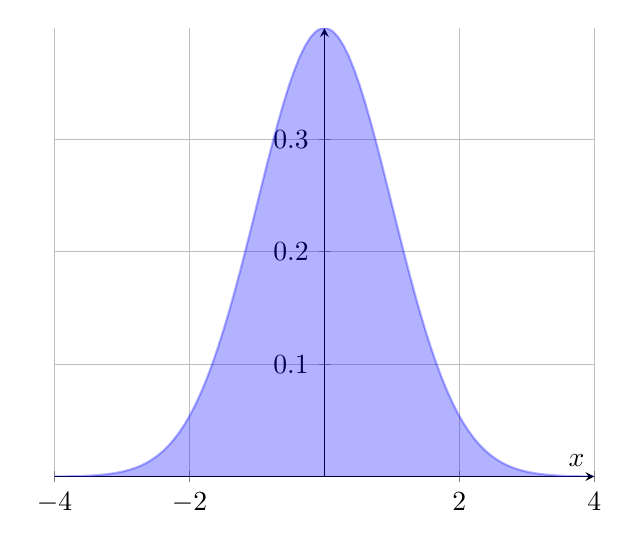
\begin{tikzpicture}
\begin{axis}[
    axis lines = middle, % Adds axis lines in the middle
    xlabel = {$x$}, % Label for x-axis
   , % Label for y-axis
     % Title of the plot
    enlargelimits, % Avoids cutting off part of the curve
    domain=-4:4, % Range of x values
    samples=100, % Number of samples to generate for the plot
    axis y line=middle, % Places the y-axis in the middle
    axis x line=middle, % Places the x-axis in the middle
    grid = major, % Adds grid lines
    ]
    % Plot the normal distribution
    \addplot [
        thick, % Line thickness
        blue, % Line color
        fill=blue, % Color of the shaded area
        opacity=0.3 % Transparency of the shaded area
    ]
    {1/sqrt(2*pi)*exp(-x^2/2)}; % Normal distribution formula

\end{axis}
\end{tikzpicture}
\end{center}
Quando X segue uma distribuição normal, podemos calcular a probabilidade de X por integral ou pela tabela (tabela de distribuição normal padrão):\\



\end{document}